\chapter{Design}

\label{ch:design}

In this chapter we are going to implement the formuli presented in the previous chapter in the MaxMSP software. Additionally, we are going to structure some other effects and variation on the context of the Phase Vocoder.

We will present the MaxMSP function that encapsulate mathematical functions like FFT, IFFT and other transformations. One can expect to fully understand the majority of the spectral tools that MaxMSP offers to the user. At the same time we will construct an efficient series of tools to build a simple Phase Vocoder.

Dans ce chapitre nous allons réaliser les théories discutées, dans le chapitre précédent (No. 2). La réalisation des notions théoriques vont être implémentées dans le logiciel MaxMSP. L'implémentation de la théorie nous permettra de la comprendre profondément et aussi de la découvrir 

\section{MaxMSP Objects}

In this section we will mention some of the basic MaxMSP spectral objects that are delivered directly by the programm and we will analyze their functionality.

In MaxMSP exist 3 categories of objects : 1) the logical objects that logical expressions and calculi, 2) the signal objects, for signal processing, that are usually followed be a $\thicksim$ indication after their name, 3) and the Jitter objects that are used for multidimensional data.

The way the spectral object work in MaxMSP is somewhat different from the rest signal objects. They are deployed in a special environment called $PFFT\thicksim$. In this environment as the name suggest an FFT is performed and because the objects deal with 2-dimensional data they are treated in a different patch\footnote{In MaxMSP a code file is called a patch among users}.

\subsubsection{$FFT\thicksim$}
    The $FFT\thicksim$ object belong to the signal family as the $\thicksim$ indicator suggests. It's the object that performs Fast Fourier Transform. It has no inputs and three outputs one for the real part of the exponential, one for the imaginary part and one counter that keep in track of the frequency bins.

    In the usual windowed Fourier transformation :

    \begin{equation}
        X_k = \sum_{n=0}^{N-1} x_n \; e^{-j \frac{2 \pi k n}{N}}
    \end{equation}

    Where k is the index of the bin and the corresponding complex coordinates are $\sum_{n=0}^k x_n + cos(2 \pi t) $ for the real part and $\sum_{n=0}^k x_n + j sin(2 \pi t)$ for the imaginary. Of course the corresponding reduction of calculative ramification is applied by the FFT algorithm discussed in previous chapter.


\subsubsection{$IFFT\thicksim$}
    Similarly the inverse FFT is treated by the appropriate object function with the inverse inputs and outputs.

\subsubsection{$cartopol\thicksim$}
    Usually is not that helpful to use this Cartesian coordinates, produced bu the $FFT\thicksim$ corresponding to the real and the imaginary part in the $\mathbb{C}^2$plane. Therefore an object that transforms Cartesian coordinates to a polar form called $cartopol\thicksim$ is frequently deployed. This object takes of course two inputs(real and imaginary) and outputs a phase and a magnitude.

\subsubsection{$poltocar\thicksim$}
    Exactly the inverse function from $cartopol\thicksim$.

\subsubsection{$FFTinfo\thicksim$}
    The $FFTinfo\thicksim$ is very frequently used and it reports information about the FFT parameters such as the size of the window, etc.
\subsubsection{$framedelta\thicksim$}
    A very important object as it computes the phase derivation between successive FFT frames. 

\subsubsection{$gen\thicksim$}
    An object that creates a new patch window. In the $gen\thicksim$ object the user can use a new set of functions that specialize single sample treatment. The functions are relatively simpler than the usual coding environment but one can do a more precise work on details. Is frequently used to perform one sample delay creating a low-pass filter or similar effects

\section{Pitch tracking}

Using some of these MaxMSP spectral objects we are going to start by building a simple pitch tracker :

    \begin{displayquote}
        '' Frequency domain pitch detection methods dissect the input signal into frequencies that make up the overall spectrum. The spectrum shows the strength of the various frequency components contained in the signal. The goal is to isolate the dominant frequency, or "pitch" out of the spectrum ''. \footnote{Curtis Roads, \textit{The Computer Music Tutorial, 1996, p. 513, op. cit}, \nocite{Roads:1996:CMT:525484}}
    \end{displayquote}

Likewise we implemented a MaxMSP patch to find the dominant frequency of the FFT window. The patch can be find in figure \ref{PitchTracking}.

%L'analyse spectrale est essentiellement  un outil qui permet de relever les composants d'un son et, par conséquent, les fréquences et les amplitudes de ses harmoniques\footnote{\citealp*[]{Dol86}}. En ce qui concerne la détection de la fréquence dominante, j'ai implémenté le patch présenté sur la figure \ref{PitchTracking}.

    
    \begin{figure}
        \centering
        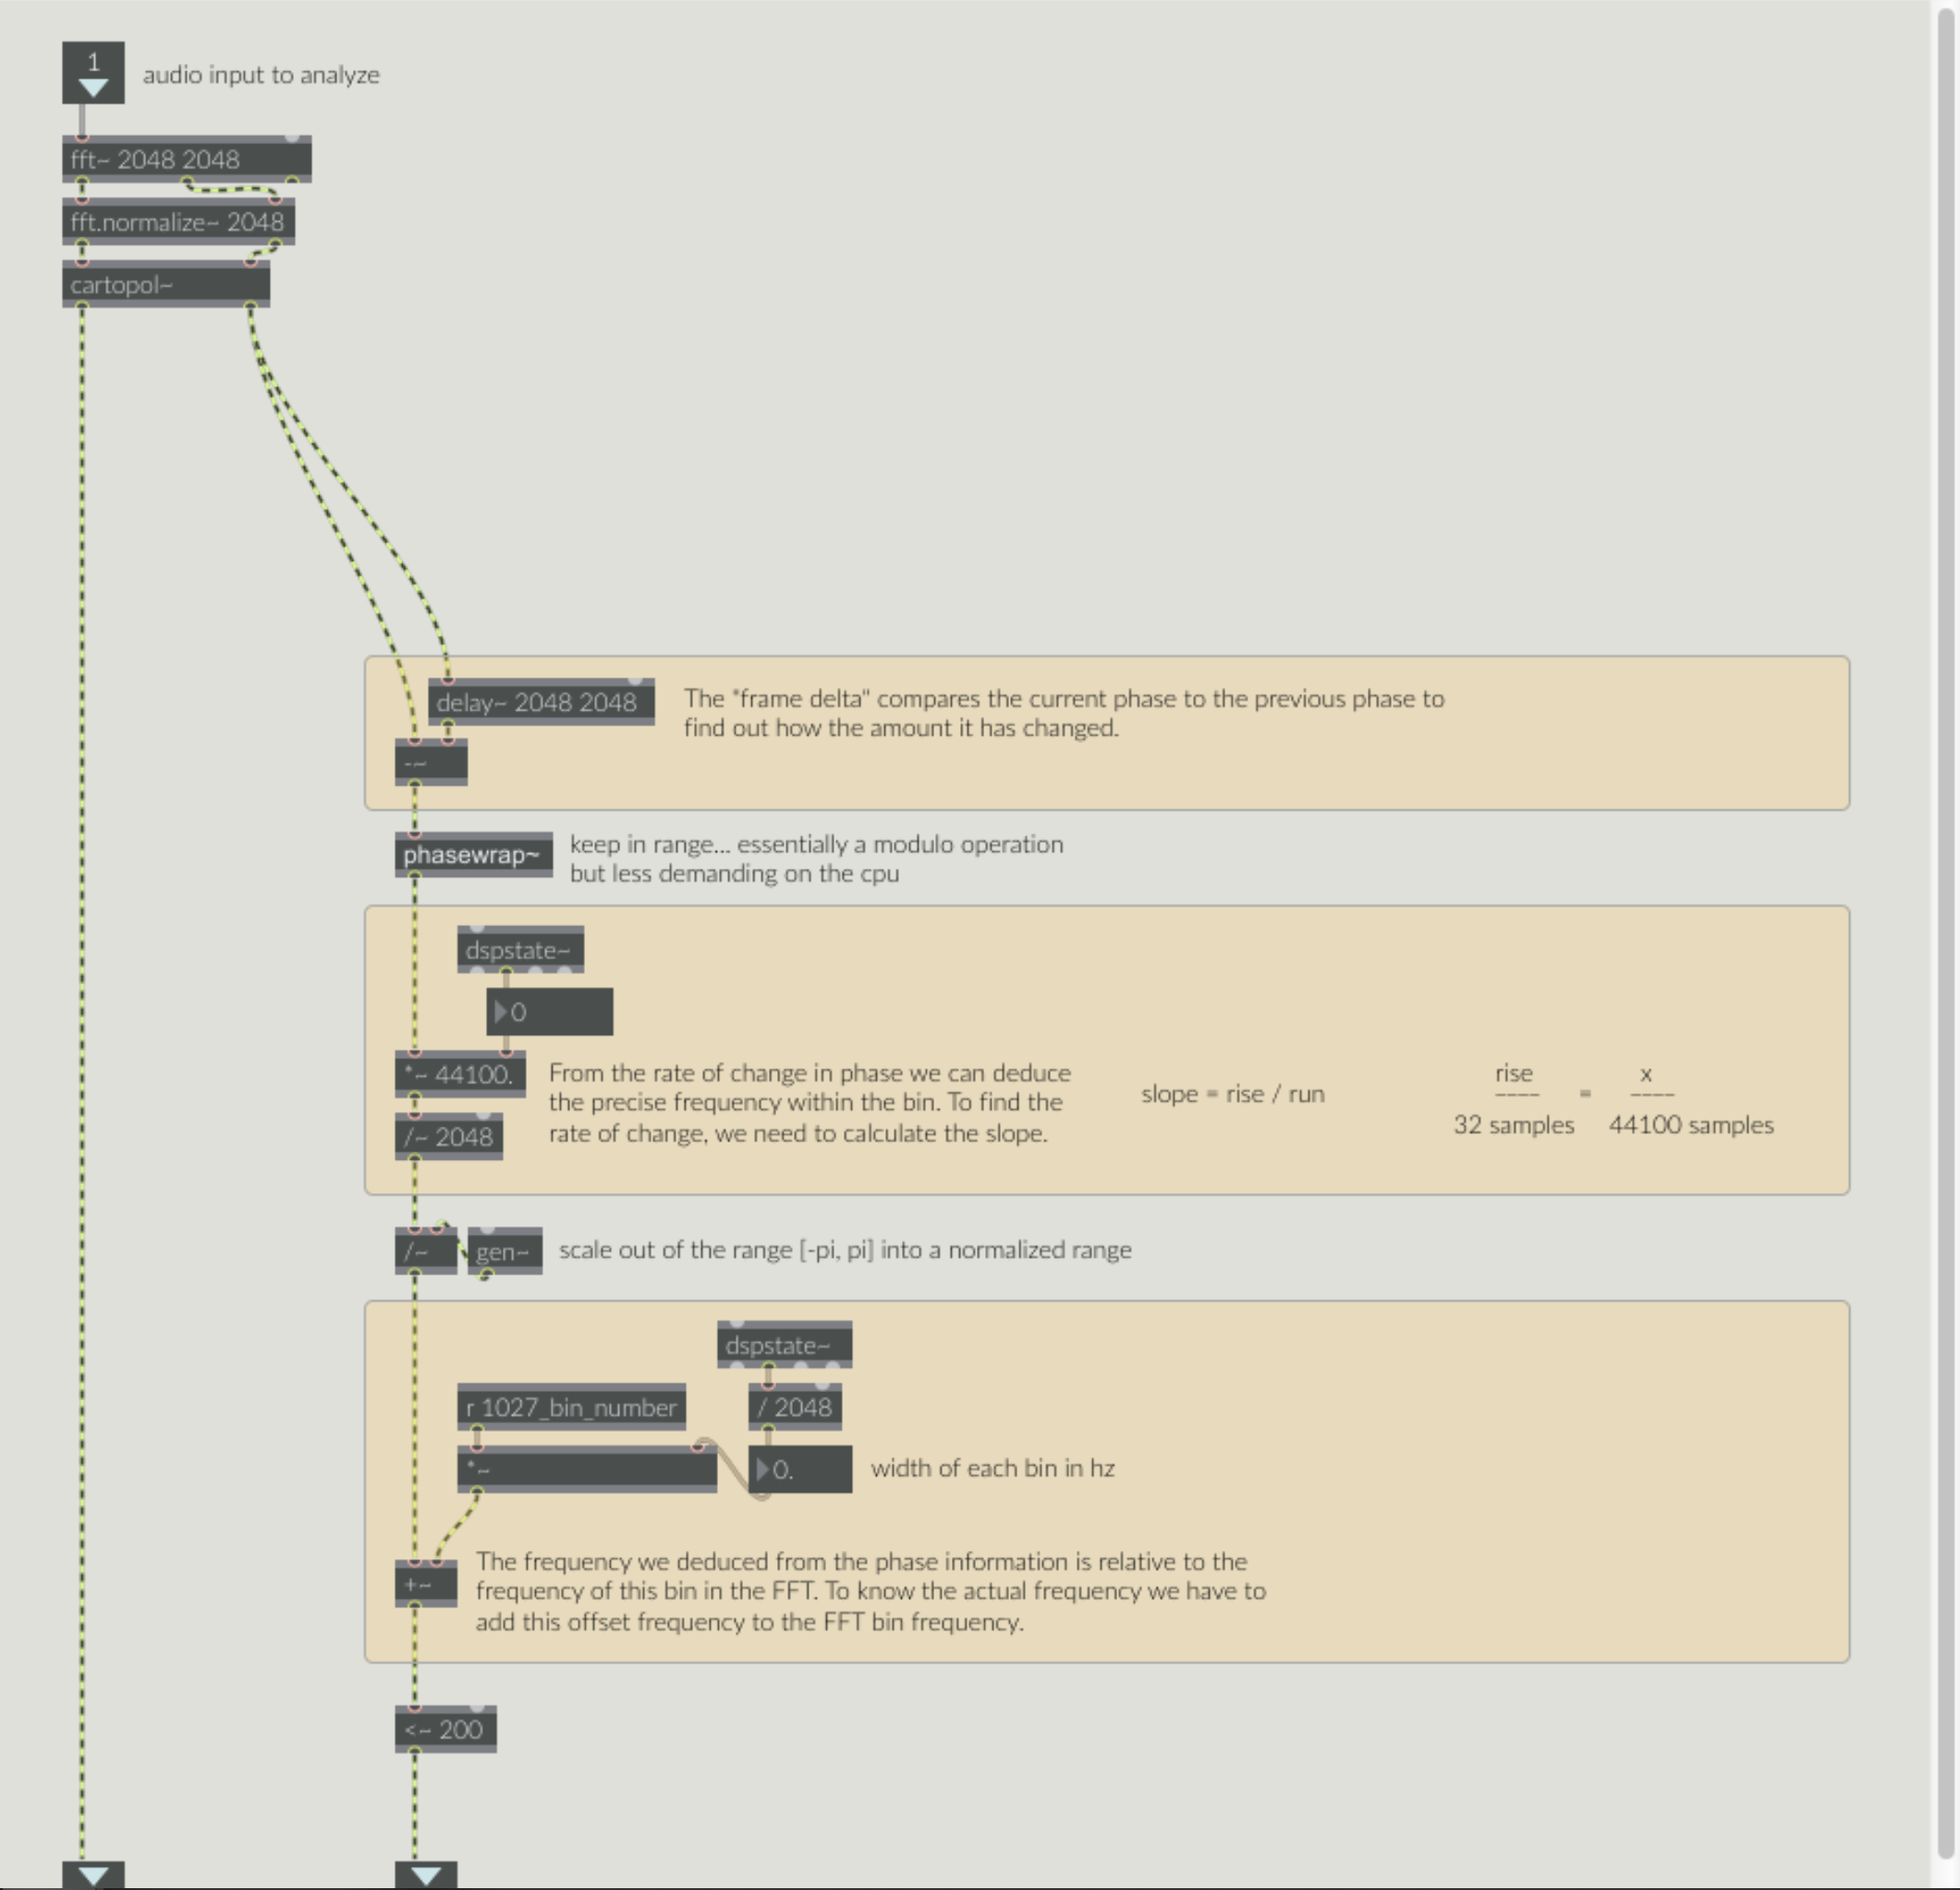
\includegraphics[width = \textwidth ]{Graphs/fftTrack.png}
        \caption{Pitch Tracking}
        \label{PitchTracking}
    \end{figure}
As expected, we use the object $fftin\thicksim$ to transform in to the frequency domain. In the FFT we have to declare two things. First the number of frames objected to FFT and second the size of the window. We remind that the first two outputs yield the real and the imaginary components respectively. The third output yields the indexed frequency bin taking corresponding values from $0$ to $N$, where $N$ is the size of the FFT window.

To continue the simple pitch tracking patch, we normalize the real and the imaginary components to restrain the data flow within computable limits. In more detail, $fft.normalize\thicksim$ is a simple Max external, created in C++ code using the Max SDK, that divides the number of each output by half the size of the window. 

Thereafter, we transform cartesian coordinates to polar using $cartopol\thicksim$. The process is explained in section 2 under the terms phase and magnitude. We are only interested on the phase of each bin. Using phase we can calculate the exact frequency of each harmonic. We remind that the terms harmonic, bin and Fourier frequency are the same in this context.
First we delay the phase of every bin by an entire window to compute the change amount. Then we substract the current phase of every bin by the corresponding phase of the previous window. Hereafter, we use the object $phasewrap\thicksim$ to clip the value range between $-\pi$ and $\pi$. It's essentially a modulo function to keep the values within a computable range. 

At this point we have to advise our sound settings. An object in Max called $dspstate\thicksim$ retrieves all the necessary data we can find in $/Options/Audio_Status$ within the Max Application. We only need the sample rate frequency. This value is usually $44100Hz$ thus we already have stored the value and if different we change it automatically. The signal obtained from $phasewrap\thicksim$ is multiplied with the sampling frequency and consequently devided by the size of the window. These operations, dividing the SR by the size of the window, deduct weighted partitions of the spectrum. The value of the frequency subtraction ranks the deviation of the frequency partition. After, we normalize by multiplying with $2\pi$ stored in a $gen\thicksim$ object. We find the position of the partition by multiplying the value of the spectrum division with the index of the bin and adding it to the deviation yields the frequency of the bin.

The spectrum devision or the partition is given by :
    \begin{equation*}
        x = \frac{SR}{\text{window size}}
    \end{equation*}
Then, the frequency is simply : $index * x + $ the phase deviation.

This procedure generates all the frequencies of all the bins of the FFT window.


%Le premier objet utilisé, appelé fftin \thicksim, transforme le signal en domaine fréquentiel. Il s'agit essentiellement d'une fonction qui effectue une transformation de Fourier rapide (FFT) et donne trois sorties. Il est nécessaire de déclarer à chaque fois qu'une fenêtre représentant le nombre d'échantillons négligés dans une analyse de Fourier. Le deuxième aspect à déclarer, est l'enveloppe de la fenêtre afin d'éviter les cliques et les pics. Les deux premières sorties représentent le vecteur d'amplitude dans un système d'axes cartésien bidimensionnel. La troisième sortie permet de fournir l'index de la corbeille d'échantillons.
%Pour poursuivre la procédure, il est crucial de normaliser les données, afin que le flux de données réel ne soit pas hors de la plage souhaitée. Ce processus est réalisé avec l'aide de l'objet fft.normalize. Il est cependant toujours nécessaire de déclarer la taille de la fenêtre comme avant.

%Les données sont traitées après leur transformation en informations plus utilisables. Ainsi, avec l'objet cartopol \thicksim, le vecteur de l'amplitude est transformé en sa forme polaire. Cette transformation se produit pour chaque index de bin. Cet objet sort la magnitude et la phase de chaque index.

The next step is to keep the frequency with the highest magnitude. We are going to use a $gen\thicksim$ object. First we declare the inputs. We only need three variables. The magnitude of each bin, the index of each bin and the size of the FFT window. We declare one single output for the strongest bin of each window. The patch is shown in figure \ref{GenSingle}.

To compute the strongest bin, we are going to use an object called $codebox$. $Codebox$ is a object that allows the user to input code in the ''traditional'' form. Just like javascript code, we have to declare the variables we are going to use but first the inputs of the object. The variables in this case are: magnitude, index, frameSize and last. Where frameSize is the FFT window size and last is just a variable that store the index of the strongest bin for the previous window.

The process of defining the strongest bin is implementated by two nested if functions. For every window this process is going to be repeated and it will determine eventually the frequencies of the strongest bins across all windows. In the nested if loop we determine if the current index is stronger than the previous one and we return the result. This means if the magnitude of the $n-$th index is a bigger value than the magnitude of the $(n-1)-$th bin, we store its index value. The last step is to restrict the number of the indexes within the limit of the window size, in order to terminate the loop and re-initialize the variables.

    \begin{figure}
        \centering
        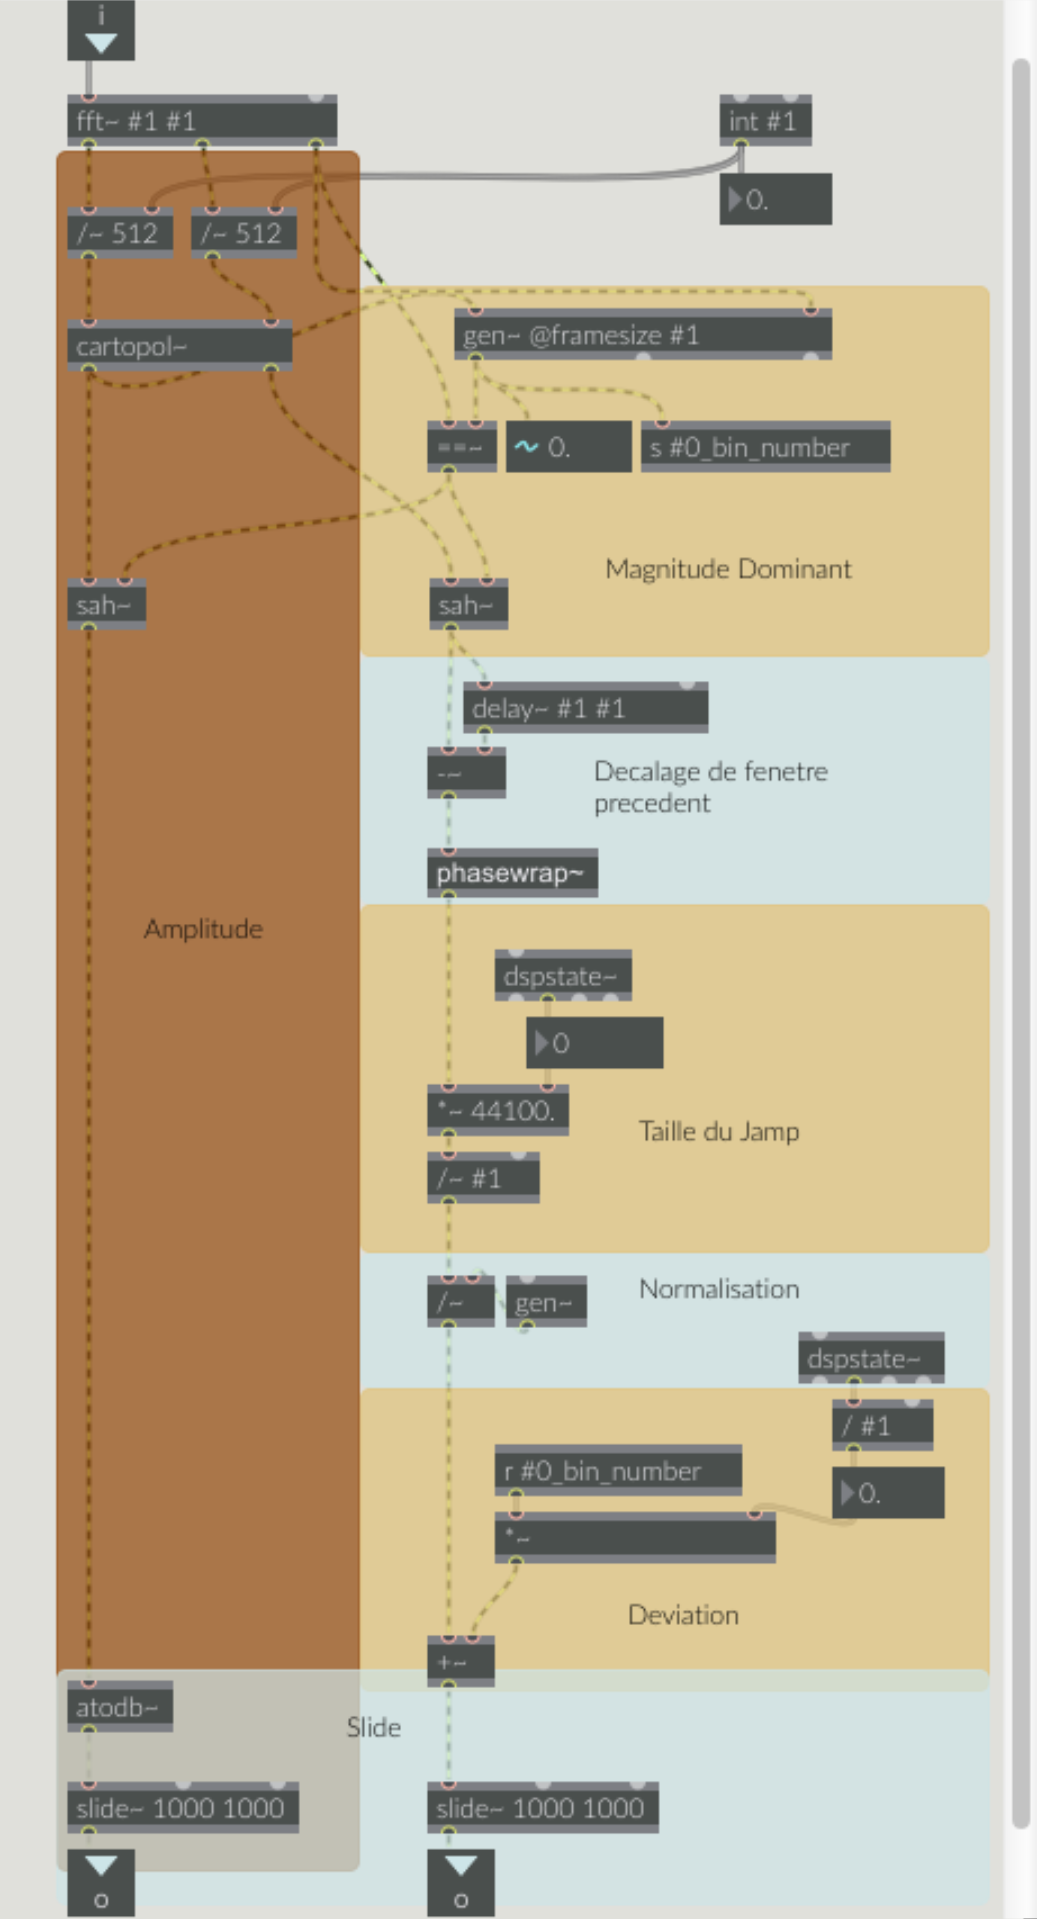
\includegraphics[width = \textwidth ]{Graphs/ffttracker.png}
        \caption{Pitch Tracker}
        \label{PitchTracker}
    \end{figure}

To track the stronger pitch a few more functions are required. The output of the $gen\thicksim$ object is filtered by a $sah\thicksim$ object. Before that, the current index is compared with the index value outputted by the $gen\thicksim$ object. $Sah\thicksim$ stands for ''sample and hold''. This function filters the first input of the object by a factor similarly to the $gate\thicksim$ object. Every time the factor value changes it allows the first input to go thought and outputs its value. We use it twice, once for the magnitude and once for the phase. This way only the index of the bin with the strongest magnitude goes thought along with the corresponding magnitude and phase. We use the system provided earlier to find the exact frequency and we translate the magnitude's polar coordinates to dB. Last but not least we use a $slide\thicksim$ object to smooth the result. The final patch is shown in the figure \ref{PitchTracker}. This method avoids computing every time the frequency if the sound is periodic and thus the dominant frequency does not change.


\subsection{Multiple Pitch Tracking}

To build a multiple pitch tracking patch we use the single pitch tracking method with a few modifications. The majority of the computations occurs within the $gen\thicksim$ object as the $codebox$ implementation is copied accordingly to the number of pitches one wishes to calculate.

    \begin{figure}
        \centering
        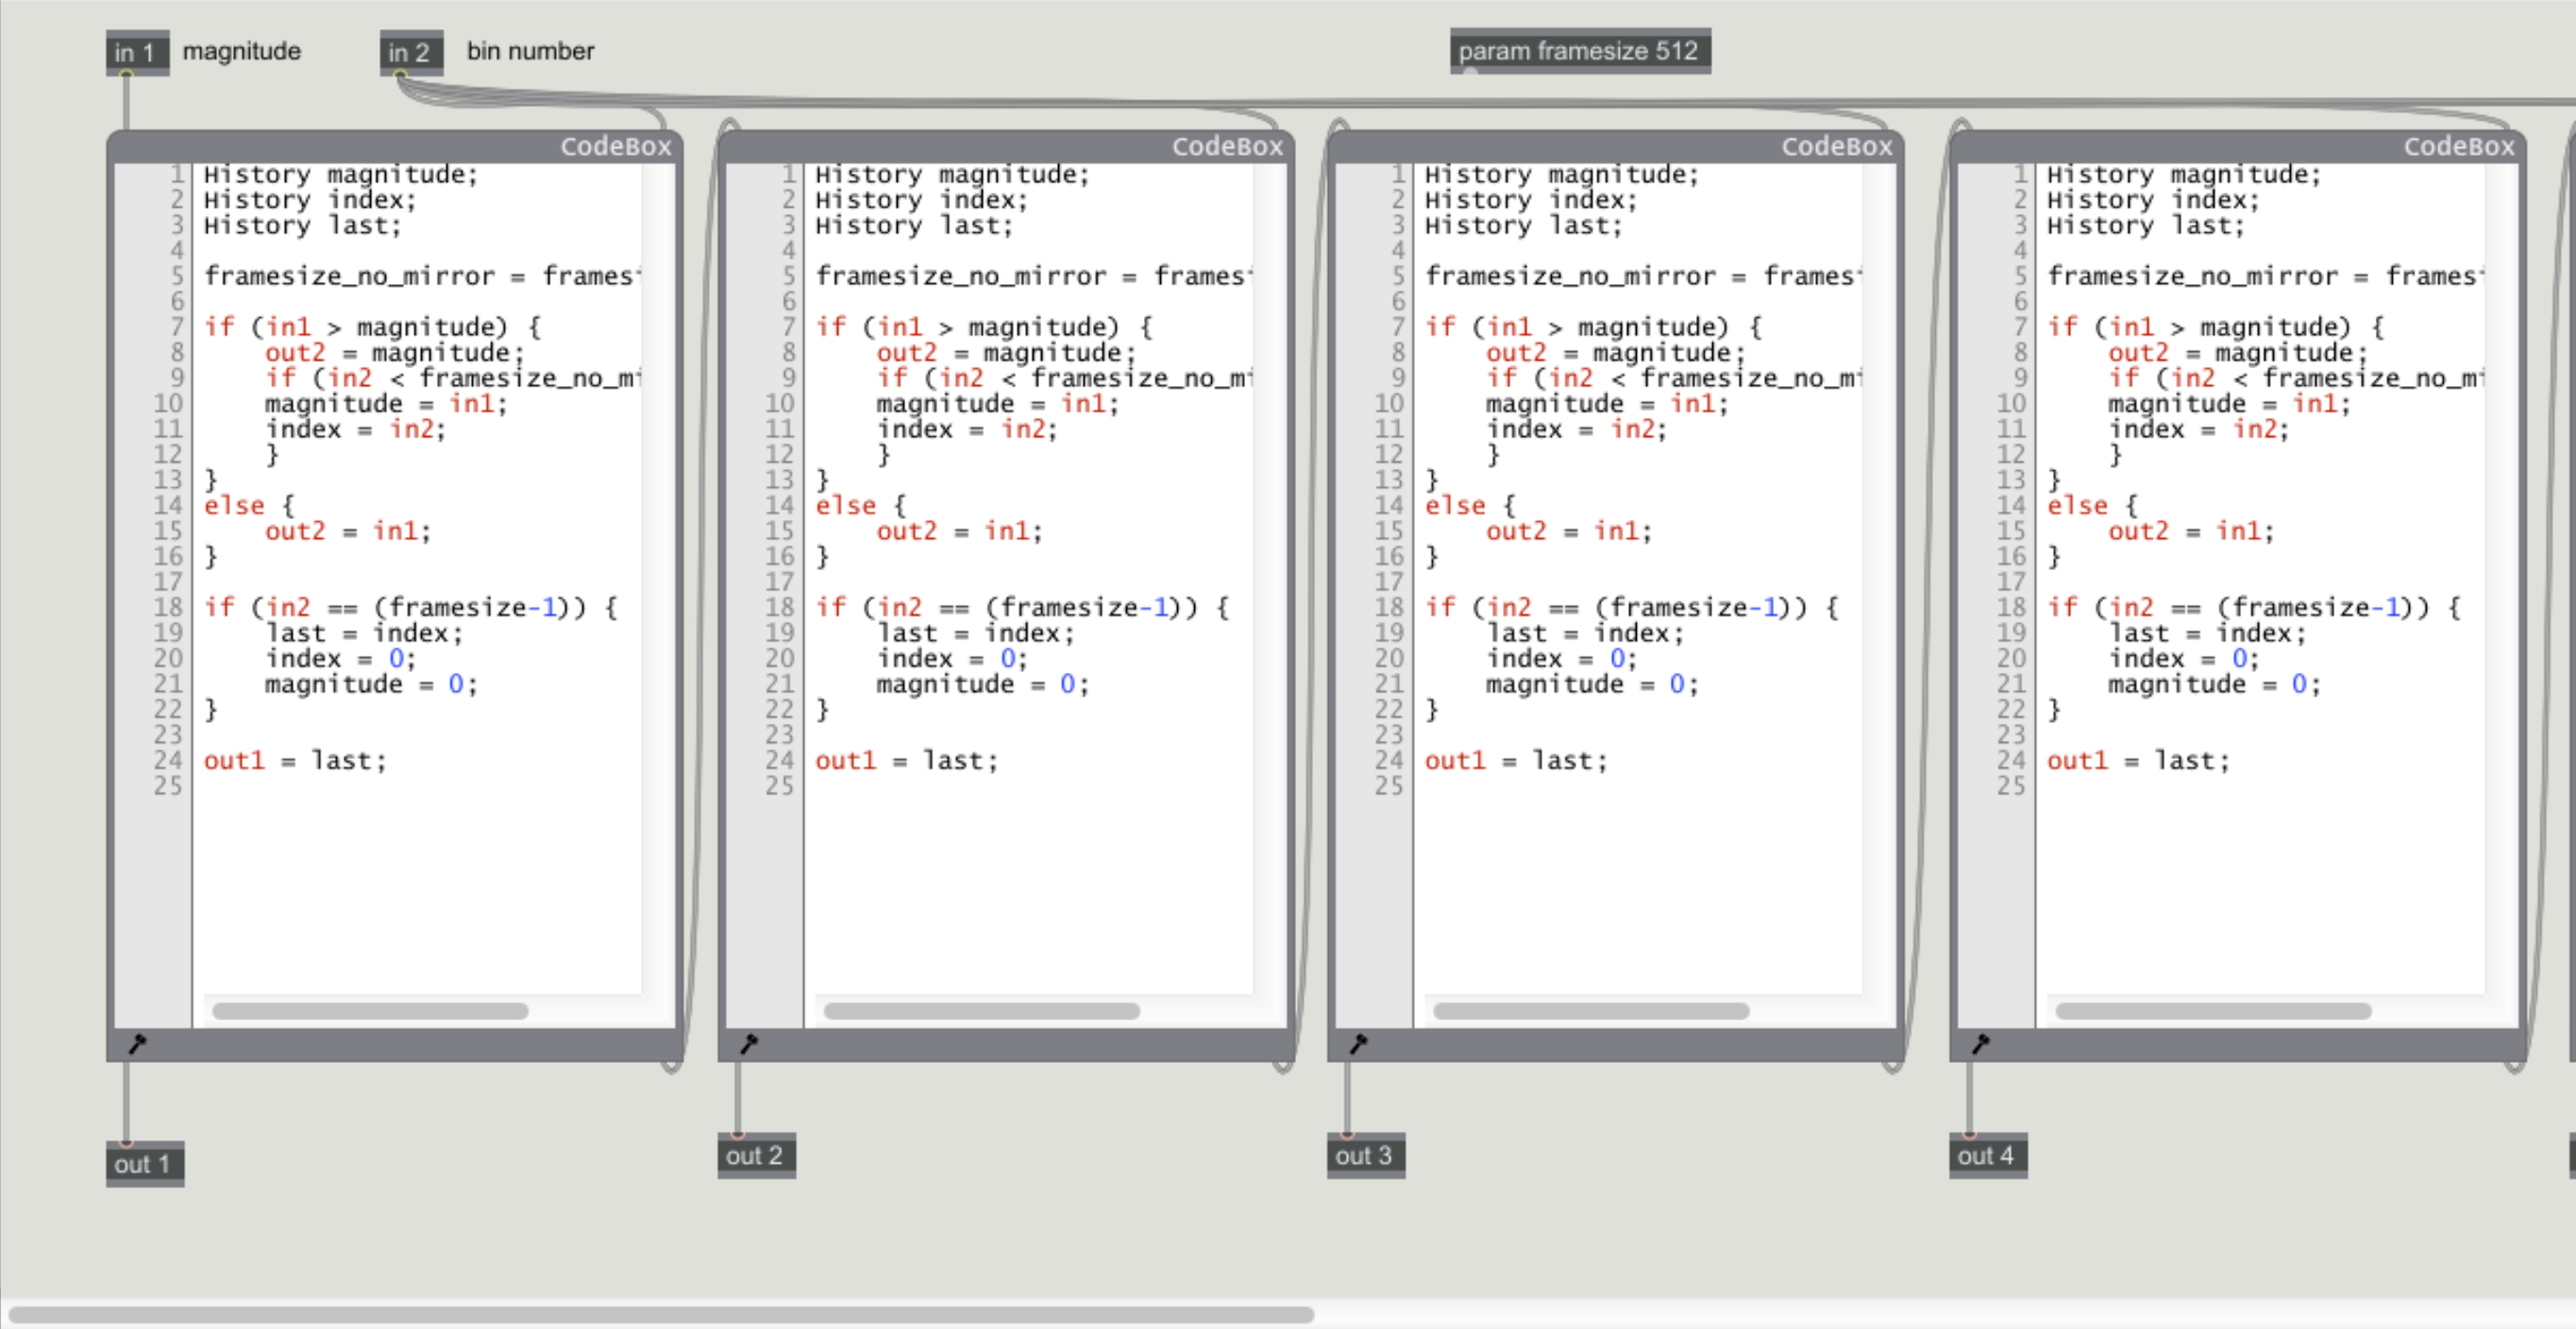
\includegraphics[width = \textwidth]{Graphs/GenMultiple.png}
        \caption{Gen multiple}
        \label{GenMultiple}
    \end{figure}

The figure \ref{GenMultiple} allows to visualize how one can compute a series of the strongest harmonics of each window. The goal is to give sufficient amount of information about the basic spectral components of sound.

As the figure \ref{GenMultiple} suggests, the output of each $codebox$ is the input of the next one thus computing the next loudest index of the window. The quantity of $codebox$ objects used relates to the number of pitches that we are going to output.

An implementation of the multiple pitch tracking method can be shown in figure \ref{Analysis}. Essentially we reproduce the frequency computation for each index. The result can be outputted either as a list or in different outlets. Then one can use the $mc.cycle\thicksim$ object, simple oscillators or resonators.

    \begin{figure}
        \centering
        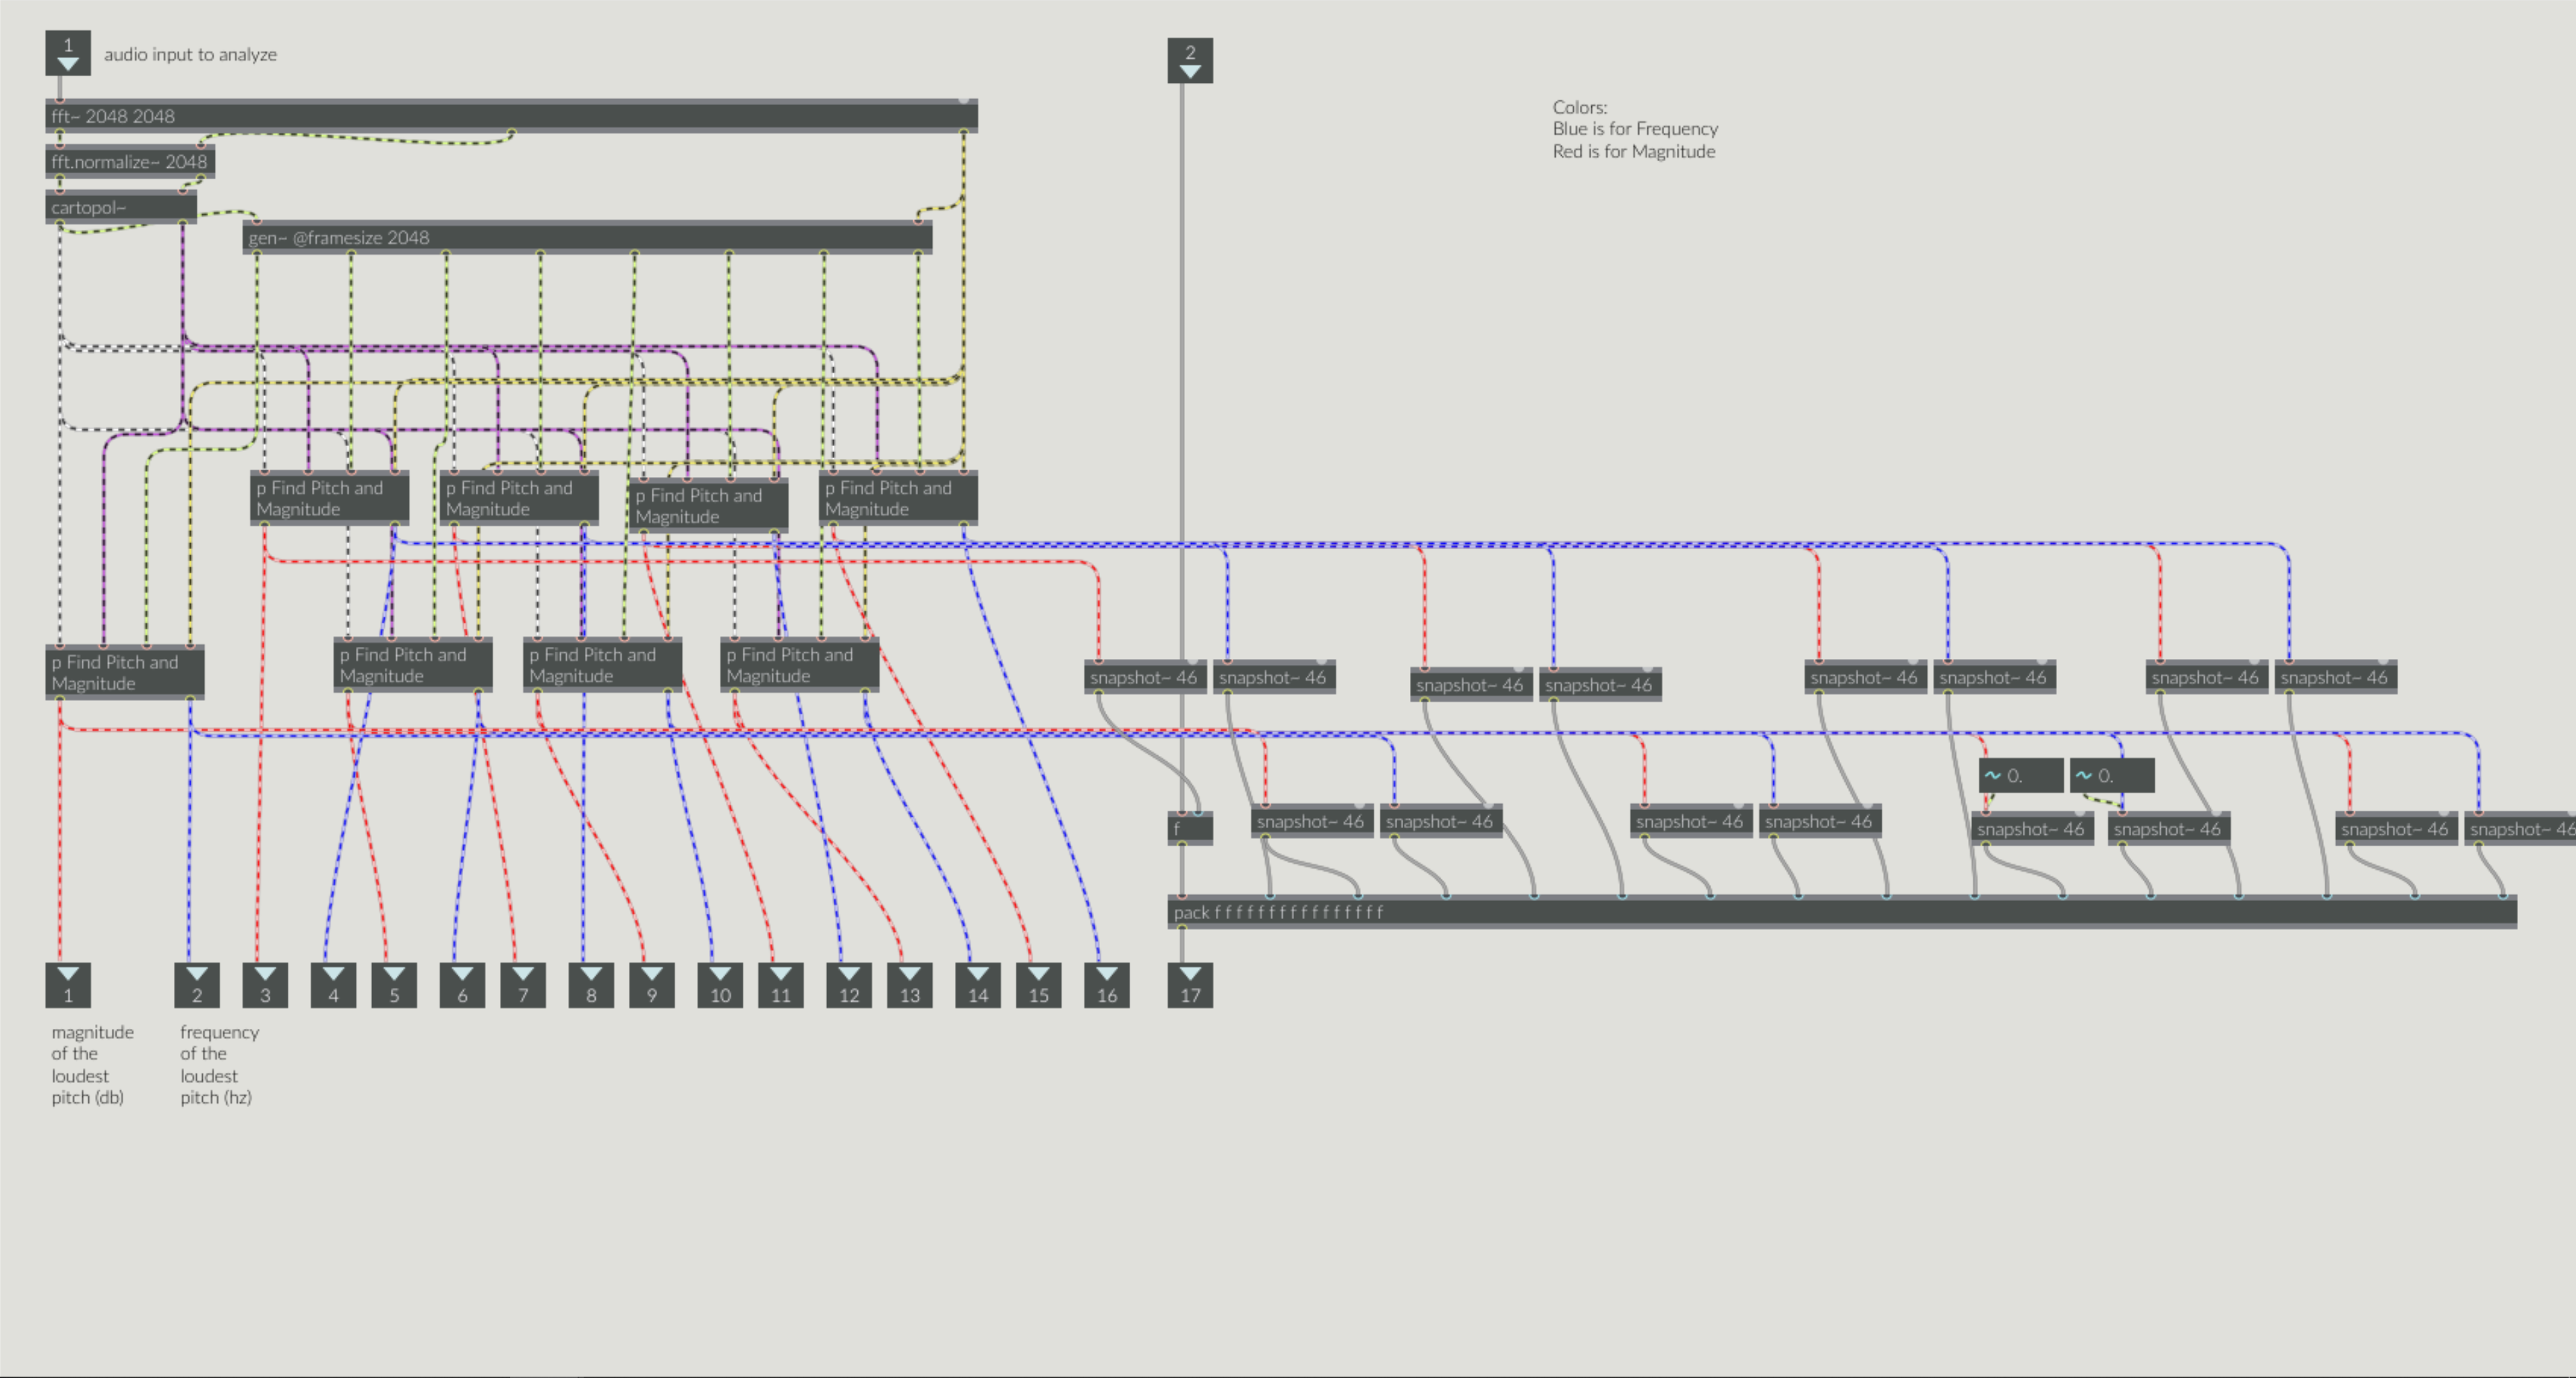
\includegraphics[width = \textwidth]{Graphs/MultipleTrack.png}
        \caption{Multiple Pitch tracking}
        \label{Analysis}
    \end{figure}

An important notice for this patch construction but also for every pitch tracking via spectral methods is that the size of the window affects the frequency tracking. The window size influences the temporal or frequency resolution of the representation of the signal. The frequency resolution can be increased changing the FFT size, that is, the number of bins of the analysis window. In particular, the size of the bins is simply the half of the analysis window. The frequency range is defined as the division of the SR to the window size\footnote{Coralie Diatkine, \textit{AudioSculpt 3.0 User Manual}, 2011 \nocite{Audiosculpt}}.

    \begin{equation*}
        Frequency \; Range = \frac{SR}{Window \; Size}
    \end{equation*}

\section{Le vocodeur de phase}

The phase vocoder was used originally for pitch transposition and changing playback speed. Likewise, we are going to build our phase vocoder on the basic model and then we are going to propose some modifications. The phase vocoder is labeled under spectral processing thus is going to be stored in a $pfft\thicksim$ object.

In order to access a sound directly into the pfft buffer one must avoid using the presets of the $pfft\thicksim$. Therefore we are going to avoid using the object $fftin\thicksim$ instead we are going to an object $fft\thicksim$ in a subpatch. The only differences is that the parameters of the $fftin\thicksim$ and $fftout\thicksim$ objects are controlled directly from the $pfft\thicksim$ object and that the in and out are the first and last objects. To build a phase vocoder we need to process sound before applying the Fourier transform. One, should follow the patch provided in the figure \ref{Phasevocoder} to understand the procedure.

Le raisonnement derrière telle logique repose sur le coeur du vocodeur de phase pour l'étirement sonore et le changement de l'hauteur. Le vocodeur de phase nécessite une lecture indépendante du son à transformer pour chaque superposition de la FFT. Chaque image sonore de la lecture doit être synchronisée avec son image sonore respective de la FFT. Par conséquent, une seule copie du son ne peut pas être lancée dans un objet $fftin\thicksim$, mais plutôt dans un objet $fft\thicksim$. L'objet $fft\thicksim$ exécute une FFT à spectre complet (c'est-à-dire en miroir), donc $fft\thicksim$ peut fonctionner en synchronisation avec les images consecutives de la FFT traitées dans l'objet $pfft\thicksim$ mais c'est nécessaire de faire quelques modifications sur l'objet $pfft\thicksim$ pour que il se comporte de la même manière.

Tout d'abord, l'objet $pfft\thicksim$ doit traiter des images sonore de la FFT à spectre complet, au lieu de l'image spectrale par défaut qui correspond à la moitié de la taille FFT (jusqu'à la moitié de la frequence de Nyquist). Cela se fait facilement en ajoutant un cinquième argument non nul à l'objet $pfft\thicksim$. Comme l'argument du spectre complet est le cinquième argument, nous devons fournir tous les autres arguments avant lui, y compris le quatrième argument, le début, qui sera défini sur la valeur par défaut de zéro.

Ensuite, puisque les objets $fftin\thicksim$ et $fftout\thicksim$ effectuent le calcul de la FFT à la phase zéro par rapport à la FFT (le premier échantillon de la fenêtre envoyée au FFT est le milieu de la fenêtre), et les $fft\thicksim$ et $ifft\thicksim$ objets exécutent la FFT déphasée de 180 degrés, il faut assurer que tous les objets $fftin\thicksim$ et $fftout\thicksim$ du patch ont le même décalage de phase FFT utilisé dans les objets $fft\thicksim$.

Cela peut être accompli en spécifiant un déphasage par rapport aux objets $fftin\thicksim$ et $fftout\thicksim$. Une valeur de phase de $0.5$ signifie un déphasage de $180$ degrés, donc c'est la valeur préférable dans ce cas. Bien que, le objet $fftin\thicksim$ ne soit pas volu, le objet $fftout\thicksim$ peut pratiquement être utilisé comme sortie pour l'objet $pfft\thicksim$. Le fenêtrage automatique dans l'objet $fftout\thicksim$ devrait se comporter comme le fenêtrage manuel avec les objets $fft\thicksim$.

Dans cette version du vocodeur de phase on va utiliser un son pre-determiné. Ca veut dire que on utilisera un enregistrement et on le stora dans un objet $buffer\thicksim$. Le $buffer\thicksim$ doit être accessible à deux endroits. Premierement à l'emplacement de la image sonore de la FFT actuelle et, en deuxième lieu, à l'emplacement de la image FFT précédente du $buffer\thicksim$. C'est possible d'utiliser soit l'objet $index\thicksim$ ou l'objet $play\thicksim$\footnote{L'objet $play\thicksim$ est utilisé comme interface de lecture de l'objet $buffer\thicksim$. $play\thicksim$ joue des samples en accord d'un offset parmi le buffer.} pour accéder au $buffer\thicksim$. Lorce que on precise la position de la transformation Fourier en durée courte manuellement, on doit trouver un systeme pour preciser le decalage du fenetre dans notre buffer.

La solution dans cette problematique et de utiliser deux objets $fft\thicksim$ parallels avec un decalage d'un quart. Un tel systeme permetra de calculer l'image actuelle de chaque index du fenetre en comparaison de l'index correspondant de la fentre precendant comme etait fait dans le patch du pitch tracking. Le decalage est calculé pour un distance d'un quart puisque on prend en compte le parametre d'overlap. L'objet $frameaccum\thicksim$ dans ce cas remplace la sequence des objets $phasewrap\thicksim$, et normalisation entre $\pi$ et $-\pi$ que on a construit dans le patch du pitch tracking.

Pour la synchronisation du buffer on utilise un objet $count\thicksim$ au parametres $0$, la taille du fenetrage, $1$ et $1$. Comme ca on peut trouver l'echantillon au quelle la FFT commence à la fois, ainsi que la position actuelle en durée totale du son. Chaque fois que le compter ce re-initialize au zero, un objet $sah\thicksim$ permet au valeur de passer, dont on deduit le premier sample de la FFT. en ajoutant les valuers du compter on peut deduire la position actuelle sur le fichier sonore. Le dernier nous permet de jouer le fichier à partir de un objet $play\thicksim$. 

On rappelle la formule du vocodeur de phase : 
    \begin{equation*}
    Phase \; Vocoder \; = \; \sum_{n=0} ^{N-1} h_a(n) \; x(n + uR_a) \; e^{-j \omega \frac{n}{N}} \vspace{0.5cm} 
    \end{equation*}
Dans la formule ci-dessus on peut voir que il y a un fenetrage correspondant, marqué $h_a(n)$. Pour simplifier on va substituer avec quelques parametres réels. On remplace $N$ par une taille de la fenetre à $1024$ echantillons. On etablit on decallage de 4 fois par fenetre, donc $uR_a = (\frac{1}{4} * 1024)_a$ pour l'index $a$ de la fenetre precedente. 
    \begin{equation*}
    Phase \; Vocoder \; = \; \sum_{n=0} ^{1023} h_a(n) \; x(n + 256_a) \; e^{-j \omega \frac{n}{1024}} \vspace{0.5cm} 
    \end{equation*}
À partir de cette formule on peut identifier les elements qui la reproduce dans le patch Max. On identifie les elements de la formule dans notre patch. La fonction, correspondant à la phase de l'analyse, contient la somme des echantillions du signal qui appartiennes à la taille de la fenetre de la FFT plus des echantillions qui appartiennes $\Sigma_n (x_n) $ à la fennetres decallée par la taille \textit{hop}, $uR_a$. Les echantillions sont multipliées, d'abord, par une fenétrage $h_a(n)$ et ensuite par la formule de Euler qui equivaute à la transformation de Fourier.

    \begin{figure}
        \centering
        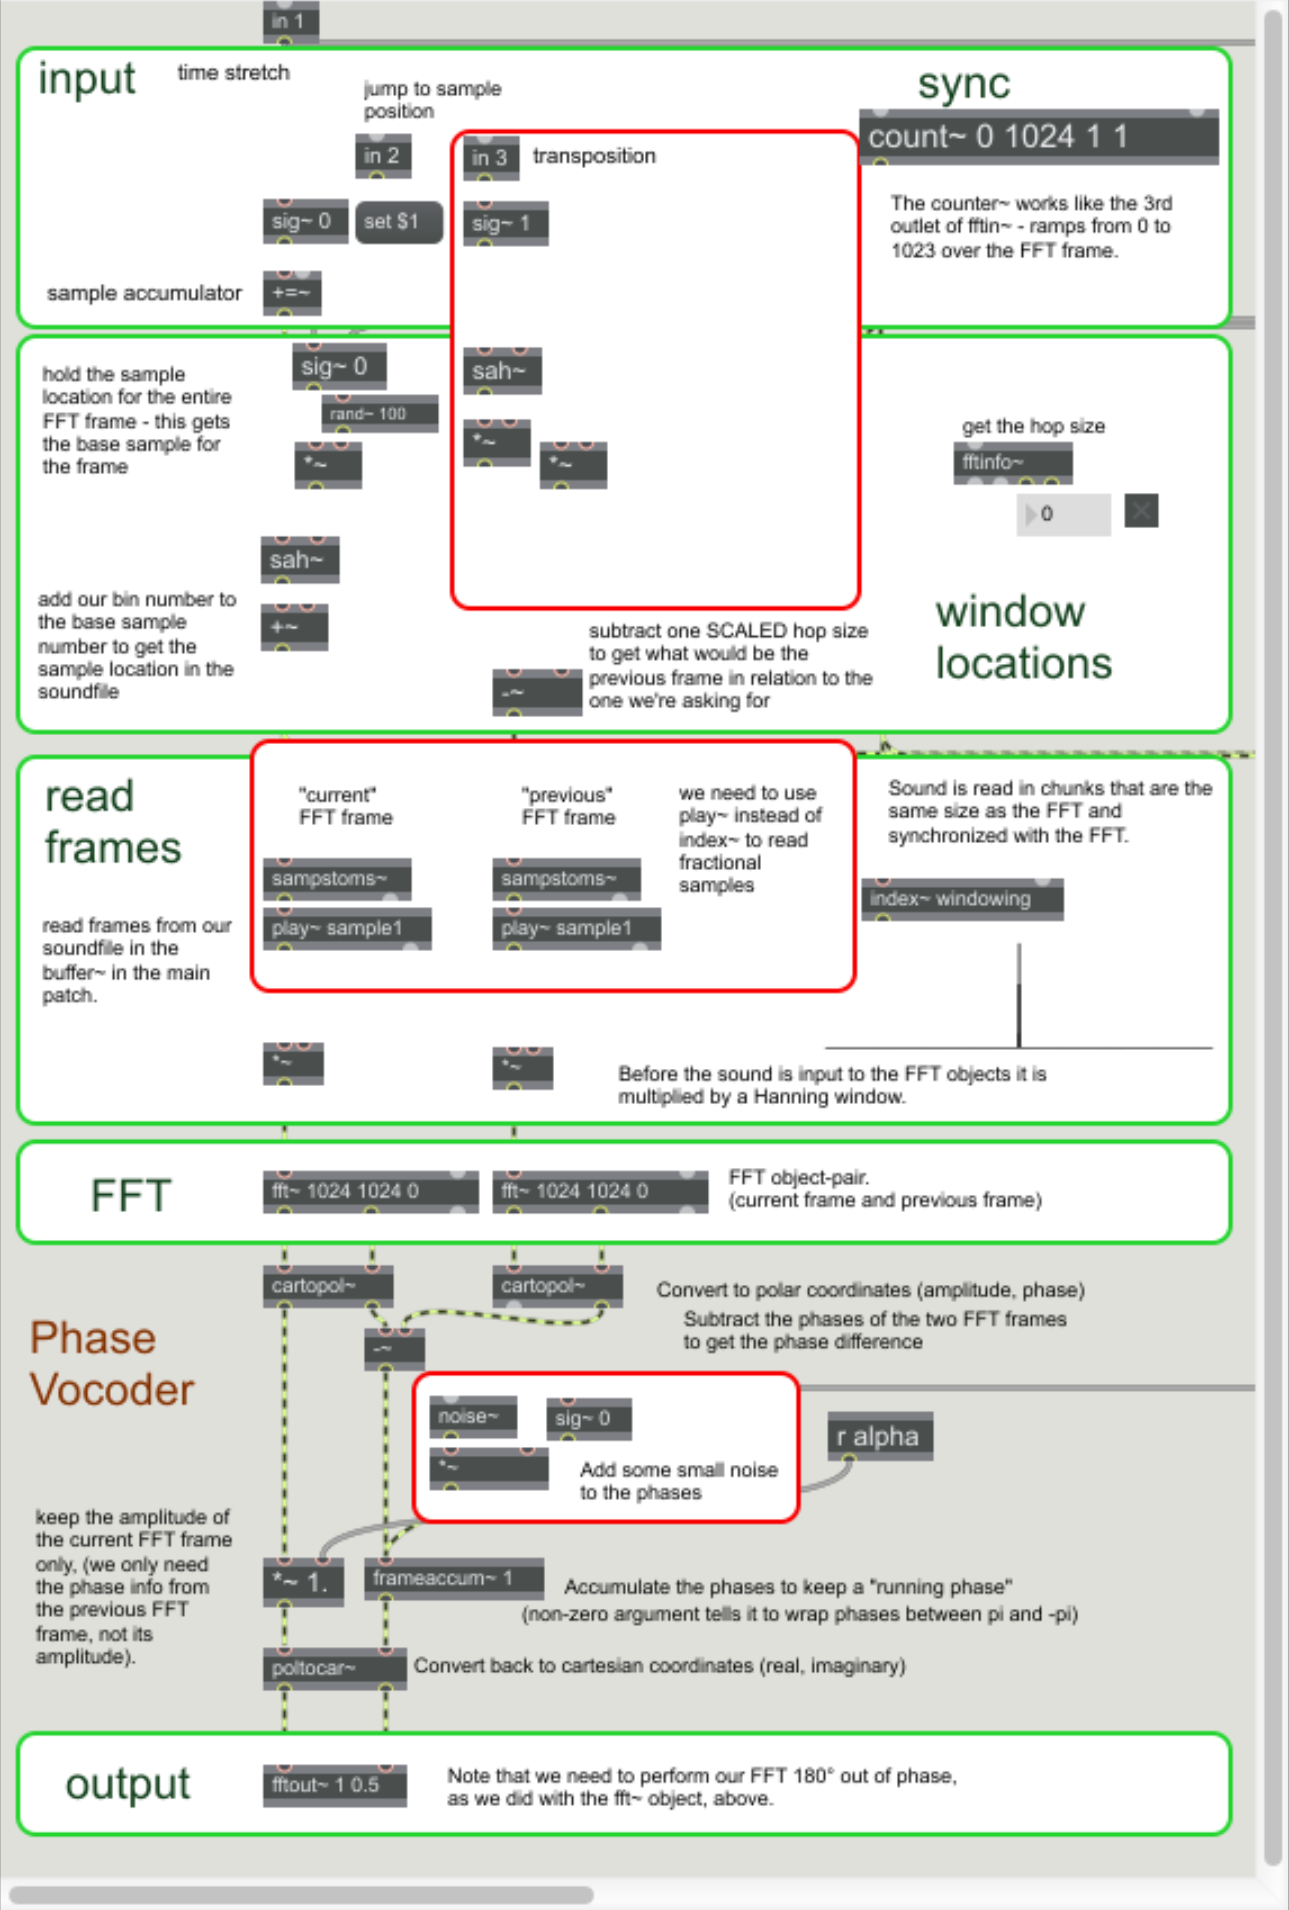
\includegraphics[width = \textwidth]{Graphs/PhaseVocoder.png}
        \caption{Le vocodeur de phase}
        \label{Phasevocoder}
    \end{figure}
    
We can see that a windowing feature is including both in the formula and in the patch presented. Instead of using a default windowing from the $fft\thicksim$ object, we are going to use a fixed buffer of $N$ size and using the $count\thicksim$ object we are going to access each sample with the assistance of the $index\thicksim$\footnote{The object $index\thicksim$ is used to read from a $buffer\thicksim$ object at a signal-driven sample index with no interpolation on the output.} object and multiply it with the sound we want to process before performing the FFT. 

\subsubsection{Filtre Gabor}

In section 2 we presented Gabor filtering. In this section, we are going to create a personalized Gabor filter. The normalized Gabor formula allows to modify the curve of the gaussian function while keeping the maximum and minimum values constants. This custom made gaussian windowing is presented in figure \ref{windowing}. 

We use an $uzi$\footnote{sends the number of banks that have been set in the argument position at once. } object with argument the size of the FFT window, followed by the expression which performs a normalized gaussian curve. Then we send it to the buffer named "windowing" with the help of the object $peek\thicksim$\footnote{The object $peek\thicksim$ is used to read and write sample values to a named $buffer\thicksim$.} Of course in this case the Gabor filter is not directly performed during the FFT but exactly before. Using this filtering we can freely overlap windows and avoid artifacts.
    
    \begin{figure}
        \centering
        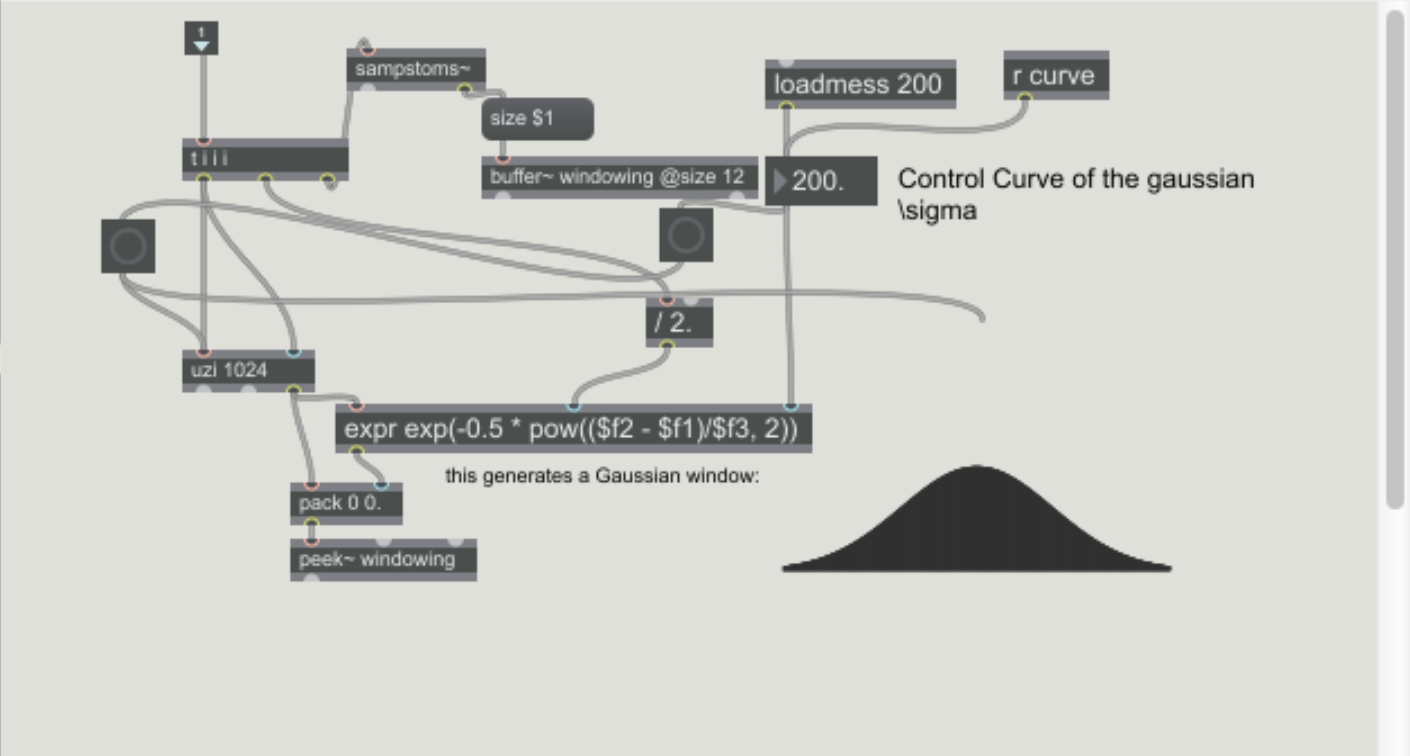
\includegraphics[width = \textwidth]{Graphs/windowing.png}
        \caption{Fenetrage gaussien}
        \label{windowing}
    \end{figure}

\subsubsection{Pitch Shifting}

    To apply pitch shifting with the Phase Vocoder one should change the pitch factor while at the same time change the sample rate. For example, in order to transpose a sound an octave lower we should playback the sound at half the speed while doubling the SR. By using this method it is possible to change the pitch with affecting the playback speed.

    To use this method we use standard midi values translated to frequency and adapted to the window overlap. The user then can input the value in a virtual midi piano thus facilitating the manipulation. By default the midi note Do with value 60 is the standard pitch. Then the pitch changes accordingly to the interval accordingly to the default value. Therefore, a Do an octave lower in the virtual midi piano, corresponds to an octave down of transposition from the original pitch of the sound.

    Inside the phase Vocoder, the pitch shifting is translated as skipping samples or oversampling the $count\thicksim$ object. Of course to increase the SR is not a valid solution thus we choose to take a smaller or larger portion from the $buffer\thicksim$ corresponding to the window size. A transposition up corresponds to taking a larger window from the $buffer\thicksim$ and reading it in a faster speed, while a pitch shift down corresponds to cutting a smaller portion of the $buffer\thicksim$ and reading it slower.

    For this example we use a $sah\thicksim$ object to make sure the transposition value is held constant for all bins during the FFT. Then we multiply with the current value of the counter and we add the output value to the number of samples played so far to get the desired location of the file. In respect of the original frequency $\omega$, the individual shift amounts to : 

    \begin{equation*}
        \Delta \omega(\omega) = \omega (\alpha - 1)
    \end{equation*}
    Where $\alpha$ is the transposition factor and $\Delta \omega $ the frequency difference. This technique imposes a constant frequency transposition $\Delta \omega$ to all the detected frequencies of the FFT.

    The Pitch shifting implementation can be viewed in the figure . It takes only a few objects to implement a pitch shifting on the basic body of the phase vocoder.



\subsubsection{Playback speed}

    As it was investigated in section 2, changing the playback speed while keeping the pitch stable is the inverse operation of pitch shifting. Playback can be controlled by taking into consideration the overlapping factor of the FFT windows. One can simply divide by the overlapping factor and add the percentage of the desired playback. Inside the vocoder the factorized value is added to the sample accumulator. On this wise, the playback speed value is added in the sample position interpretation. A faster playback skips samples where a slower playback speed read samples multiple times. The subtraction from the previous position of each sample (la window of the FFT), fixes the frequency deviations. 

\section{Morphing spectrale}

The final demonstration for this chapter is an implementation of spectral morphing or spectral cross synthesis. To accomplish this technique we use two parallel phase vocoders and we interpolate phase and amplitude of each bin index. To understand the computational complexity of spectral morphing we will remind that a simple phase vocoder uses two parallel FFTs shifted by the overlap window factor. So if we use a window of 1024 samples and a overlap factor of 4, then the first FFT starts in position $0$ and parallel window at sample position 256. Now for spectral morphing we use 4 parallel FFTs. That's a lot of computation, but still is possible with current computers.

In this double phase vocoder the outputs of the object $cartopol\thicksim$, the magnitude and the phase after the Fourier analysis, are multiplied by the morphing interpolation factor. The phase is corrected beforehand by an accumulation with the previous frame and an smalled amount noise is added for a more natural result. We separate the magnitude and phase interpolation channels. Thusly, one can prefer to output, for example, the magnitude of the source sound but the phase of the target sound. 

The output of each sound after the interpolation is transformed into Cartesian form and a inverse FFT is applied. Thus we obtain a seamless sound result. At this point a number of editing operation can be added, such as noise modeling or varying interpolation per frame, etc. But before diving into advanced modifications let us first investigate the interpolations techniques.

Interpolation is set by default to linear. A simple Javascript code we implemented creates a linear curve. The interpolation values vary between $[0, 1]$. The value $0$ corresponds to zero interpolation, thus the magnitude or phase of the source sound is outputted. A value of $1$ outputs entirely the characteristics of the target sound and omits the source sound. A linear curve sets a linear way to interpolate between sounds. But we go a step further and implement a number of curves such as exponential, logarithmic and, of course, linear. Therefore, one has different ways to interpolate between sounds based on their frequency components or the magnitude of their frequency components. All interpolations vary between the same integral $[0, 1]$. The Javascript code can be viewed in the listing bellow.

\noindent\begin{minipage}{\textwidth}
\lstinputlisting[language=Java]{Expondential.js}
\end{minipage}

The version of the phase vocoder for spectral morphing is shown in the figure \ref{Morphing}. There are two buffers one for the source and one for the target sound. The Gaussian windowing for Gabor filtering with an remote normalized curve. An interpolation knob for phase and an knob for magnitude interpolation control the interpolation factors for morphing and a noise factorizing for naturalizing the phase are implemented.

    \begin{figure}
        \centering
        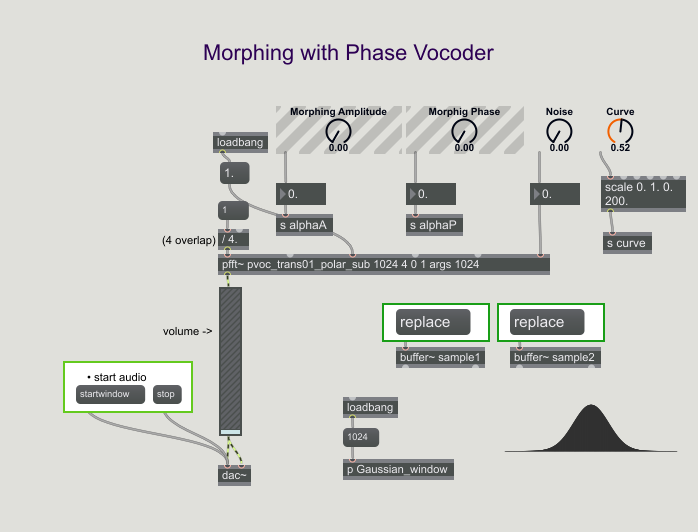
\includegraphics[width = \textwidth]{Graphs/SoundMorphing.png}
        \caption{Morphing en temps réel}
        \label{Morphing}
    \end{figure}